%%%%%%%%%%%%%%%%%%%%%%%%%%%%%%%%%%%%%%%
% Wenneker Resume/CV
% LaTeX Template
% Version 1.1 (19/6/2016)
%
% This template has been downloaded from:
% http://www.LaTeXTemplates.com
%
% Original author:
% Frits Wenneker (http://www.howtotex.com) with extensive modifications by
% Vel (vel@LaTeXTemplates.com)
%
% License:
% CC BY-NC-SA 3.0 (http://creativecommons.org/licenses/by-nc-sa/3.0/
%
%%%%%%%%%%%%%%%%%%%%%%%%%%%%%%%%%%%%%%

%----------------------------------------------------------------------------------------
%	PACKAGES AND OTHER DOCUMENT CONFIGURATIONS
%----------------------------------------------------------------------------------------

\documentclass[a4paper,12pt]{memoir} % Font and paper size

\input{structure.tex} % Include the file specifying document layout and packages

%----------------------------------------------------------------------------------------
%	NAME AND CONTACT INFORMATION
%----------------------------------------------------------------------------------------

\userinformation{ % Set the content that goes into the sidebar of each page
\begin{flushright}
% Comment out this figure block if you don't want a photo
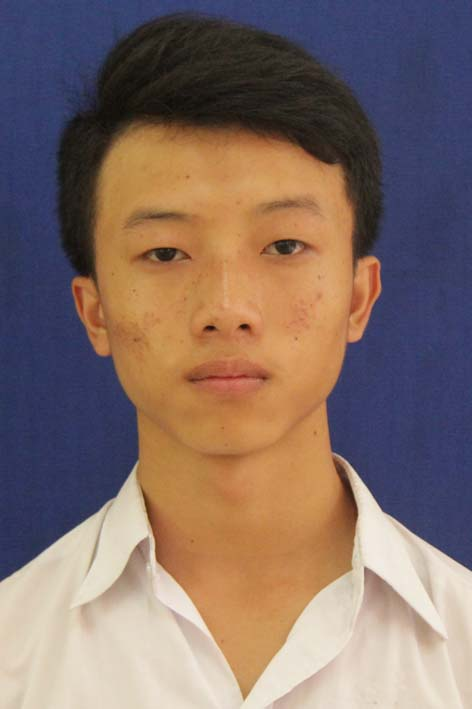
\includegraphics[width=0.6\columnwidth]{img/photo.jpg}\\[\baselineskip] % Your photo
\small % Smaller font size
Nguyen Minh Tien \\ % Your name
% 26-10-1999\\
\href{mailto:tiennm99@outlook.com}{\em tiennm99@outlook.com} \\ % Your email address
\href{https://tiennm99.github.io/}{\em tiennm99.github.io} \\ % Your URL
% (+84) 869 156 149 \\ % Your phone number
\href{https://github.com/tien99/}{\textbf{GitHub}/\em tiennm99} \\
\href{https://www.facebook.com/tiennm99/}{\textbf{Facebook}/\em tiennm99}   \\
\href{https://www.linkedin.com/in/miti99/}{\textbf{LinkedIn}/\em miti99}   \\
\Sep % Some whitespace
\textbf{Address} \\
District 7, HCMC \\ % Address 1
% \\ % Address 2
% \\ % Address 3
\vfill % Whitespace under this block to push it up under the photo
\end{flushright}
}

%----------------------------------------------------------------------------------------

\begin{document}

\userinformation % Print your information in the left column

\framebreak % End of the first column

%----------------------------------------------------------------------------------------
%	HEADING
%----------------------------------------------------------------------------------------

\cvheading{Nguyen Minh Tien} % Large heading - your name

\cvsubheading{Senior Software Engineer} % Subheading - your occupation/specialization

%----------------------------------------------------------------------------------------
%	ABOUT ME
%----------------------------------------------------------------------------------------

\aboutme{About Me}{A software architecture enthusiast passionate about building scalable systems that serve a large user base. Continuously learning from open source projects and tech blogs.
% \begin{itemize}
% \item Github: \href{https://github.com/tien99/}{\em tiennm99}
% \item Email: \href{mailto:tiennm99@outlook.com}{\em tiennm99@outlook.com}
% \item Facebook: \href{https://www.facebook.com/tiennm99/}{\em tiennm99}
% \item Linkedin: \href{https://www.linkedin.com/in/miti99/}{\em miti99}
% \end{itemize}
}

%----------------------------------------------------------------------------------------
%	EDUCATION
%----------------------------------------------------------------------------------------

\CVSection{Education}

%------------------------------------------------

\CVItem{2017 - 2023, \href{https://hcmut.edu.vn/}{\em Ho Chi Minh City University of Technology}}{
  B.E. in Computer Science - \href{https://www.cse.hcmut.edu.vn/}{\em Faculty of Computer Science and Engineering}
}

%------------------------------------------------

%\Sep % Extra whitespace after the end of a major section

%----------------------------------------------------------------------------------------
%	EXPERIENCE
%----------------------------------------------------------------------------------------

\CVSection{Experience}

%------------------------------------------------

% \CVItem{Jul 2020 - Sep 2020, \textit{VNG Tech Fresher}, Game Studio North, VNG}{
%Detailed achievements:
%\begin{itemize}
%	\item Learned how to make amazing coffee
%	\item Finally determined the reason for \textsc{PC LOAD LETTER}:
%	\begin{itemize}
%		\item Paper jam
%		\item Software issues:
%		\begin{itemize}
%			\item Word not sending the correct data to printer
%			\item Windows trying to print in letter format
%		\end{itemize}
%		\item Coffee spilled inside printer
%	\end{itemize}
%	\item Broke the office record for number of kitten pictures in cubicle
%	\item Learned how to make more amazing coffee on a new machine
%	\item Mastered the art of filing accurate TPS reports
%\end{itemize}
% Learn to make a game using Cocos2d.
% }

\CVItem{Jul 2020 - Present, \href{https://play.zing.vn/}{ZingPlay Game Studios} - \href{https://www.vng.com.vn/}{VNG Corporation}}{
Started my journey at VNG Tech Fresher Program and progressed to Senior Software Engineer at ZingPlay Game Studios (ZPS). Over the years, I have honed my expertise in game server architecture and backend development using Java, while also contributing to client-side logic with Cocos and Godot when needed. Notable projects I have worked on at ZingPlay Game Studios include:
\begin{itemize}
	\item \href{https://play.google.com/store/apps/details?id=zps.games.show}{\textbf{Show}} - A card game for Myanmar market.
	\item \href{https://play.google.com/store/apps/details?id=zps.games.burkozel}{\textbf{Burkozel}} - A card game for the Russian audience.
	\item \href{https://play.google.com/store/apps/details?id=zps.games.bida3d.vn}{\textbf{Bida3D}} - Global 8-ball pool game.
	\item \href{https://play.google.com/store/apps/details?id=vn.zps.tl2}{\textbf{Chaos Age 2}} - Global strategy game.
\end{itemize}
}

%------------------------------------------------

%\CVItem{Jan 2008 - Oct 2012, \textit{Computer Repair Specialist}, Buy More}{Worked in the Nerd Herd and helped to solve computer problems by asking customers to turn their computers off and on again.}

%------------------------------------------------

%\Sep % Extra whitespace after the end of a major section

%----------------------------------------------------------------------------------------
%	COMMUNICATION SKILLS
%----------------------------------------------------------------------------------------

%\CVSection{Communication Skills}

%------------------------------------------------

%\CVItem{2015, \textit{Oral Presentation}, California Business Conference}{Presented research I conducted for my Masters of Engineering degree.}

%------------------------------------------------

%\CVItem{2014, \textit{Poster}, Annual Business Conference (Oregon)}{As part of the course work for BUS320, I created a poster analyzing several local businesses and presented this at a conference.}

%------------------------------------------------

%\Sep % Extra whitespace after the end of a major section

%----------------------------------------------------------------------------------------
%	SKILLS
%----------------------------------------------------------------------------------------

\CVSection{Software Development Skills}

%------------------------------------------------

\CVItem{Programming}{
\begin{tabular}{p{0.4\textwidth} p{0.2\textwidth}}
    \bluebullet Java (Netty, Vert.x, Spring Boot) &  \bluebullet Javascript \\
% \bluebullet LaTeX &&\\
\end{tabular}
}

\CVItem{Databases}{
\begin{tabular}{p{0.2\textwidth} p{0.2\textwidth} p{0.2\textwidth}}
    \bluebullet Couchbase & \bluebullet Redis & \bluebullet MySQL \\
\end{tabular}
}

\CVItem{Tools \& DevOps}{
\begin{tabular}{p{0.2\textwidth} p{0.2\textwidth} p{0.2\textwidth}}
    \bluebullet Git & \bluebullet Docker & \bluebullet CI/CD \\
\end{tabular}
}

%------------------------------------------------

%\Sep % Extra whitespace after the end of a major section

%----------------------------------------------------------------------------------------
%	NEW PAGE DELIMITER
%	Place this block wherever you would like the content of your CV to go onto the next page
%----------------------------------------------------------------------------------------

%\clearpage % Start a new page

%\userinformation % Print your information in the left column

%\framebreak % End of the first column

%----------------------------------------------------------------------------------------
%	AWARDS
%----------------------------------------------------------------------------------------

%\CVSection{Awards}

%------------------------------------------------

%\CVItem{2010, \textit{Postgraduate Scholarship}, Cornell University}{Awarded to the top student in their final year of a Bachelors degree.}

%------------------------------------------------

%\Sep

\CVSection{Projects}

\CVItem{2020 - present, \textit{Static websites with Hugo}}{
  \begin{itemize}
  \item My blog on GitHub Pages - \href{https://tiennm99.github.io/}{\em tiennm99.github.io} using \href{https://gohugo.io/}{\em Hugo}.
  \item Website for \href{https://ngamtheproject.github.io/}{\em Ngăm} - a charity project founded by my brother's friends.
  \end{itemize}
}

\CVItem{2020 - present, \textit{Various personal projects showcased on \href{https://tiennm99.github.io/page/pages/}{my blog}}}{

}

%\Sep % Extra whitespace after the end of a major section

%----------------------------------------------------------------------------------------
%	INTERESTS
%----------------------------------------------------------------------------------------

\CVSection{Interests}

%------------------------------------------------

\CVItem{Professional}{Game server architecture, distributed systems, Java performance tuning}

%------------------------------------------------

\CVItem{Personal}{Reading novels \& manga, playing Genshin Impact \& TFT}

%------------------------------------------------

\Sep % Extra whitespace after the end of a major section

%----------------------------------------------------------------------------------------

\end{document}
